% !TEX TS-program = pdflatex
% !TEX encoding = UTF-8 Unicode

% This is a simple template for a LaTeX document using the "article" class.
% See "book", "report", "letter" for other types of document.

\documentclass[11pt]{article} % use larger type; default would be 10pt

\usepackage[utf8]{inputenc} % set input encoding (not needed with XeLaTeX)

%%% PAGE DIMENSIONS
\usepackage{geometry} % to change the page dimensions
\geometry{a4paper} % or letterpaper (US) or a5paper or....

\usepackage{graphicx} % support the \includegraphics command and options

\usepackage{amssymb}
\usepackage{amsmath}
%%% PACKAGES
\usepackage{booktabs} % for much better looking tables
\usepackage{array} % for better arrays (eg matrices) in maths
\usepackage{paralist} % very flexible & customisable lists (eg. enumerate/itemize, etc.)
\usepackage{verbatim} % adds environment for commenting out blocks of text & for better verbatim
\usepackage{subfig} % make it possible to include more than one captioned figure/table in a single float
% These packages are all incorporated in the memoir class to one degree or another...

%%% HEADERS & FOOTERS
\usepackage{fancyhdr} % This should be set AFTER setting up the page geometry
\pagestyle{fancy} % options: empty , plain , fancy
\renewcommand{\headrulewidth}{0pt} % customise the layout...
\lhead{}\chead{}\rhead{}
\lfoot{}\cfoot{\thepage}\rfoot{}

%%% SECTION TITLE APPEARANCE
\usepackage{sectsty}
\allsectionsfont{\sffamily\mdseries\upshape} % (See the fntguide.pdf for font help)
% (This matches ConTeXt defaults)

%%% ToC (table of contents) APPEARANCE
\usepackage[nottoc,notlof,notlot]{tocbibind} % Put the bibliography in the ToC
\usepackage[titles,subfigure]{tocloft} % Alter the style of the Table of Contents
\renewcommand{\cftsecfont}{\rmfamily\mdseries\upshape}
\renewcommand{\cftsecpagefont}{\rmfamily\mdseries\upshape} % No bold!
\usepackage{graphicx}
\graphicspath{ {./pings/} }

\usepackage{amsmath}
\DeclareMathOperator*{\argmax}{arg\,max}
\DeclareMathOperator*{\argmin}{arg\,min}

\newcount\colveccount
\newcommand*\colvec[1]{
        \global\colveccount#1
        \begin{pmatrix}
        \colvecnext
}
\def\colvecnext#1{
        #1
        \global\advance\colveccount-1
        \ifnum\colveccount>0
                \\
                \expandafter\colvecnext
        \else
                \end{pmatrix}
        \fi
}

%%% END Article customizations

%%% The "real" document content comes below...

\title{Macro PS2}
\author{Michael B. Nattinger\footnote{I worked on this assignment with my study group: Alex von Hafften, Andrew Smith, and Ryan Mather. I have also discussed problem(s) with Emily Case, Sarah Bass, and Danny Edgel.}}

%\date{} % Activate to display a given date or no date (if empty),
         % otherwise the current date is printed 

\begin{document}
\maketitle

\section{Question 1}
In this question we will model a 2-dimensional linear system, the Ramsey model of consumption and capital. We have the following:
\begin{equation}
k_{t+1} = zk_{t}^{\alpha} + (1-\delta) k_t - c_t \label{eqn:kap}
\end{equation}
\begin{equation}
\frac{\beta}{c_{t+1}} = (c_t)^{-1} (1 - \delta + \alpha z k_{t+1}^{\alpha - 1})^{-1}  \label{eqn:con}
\end{equation}
\subsection{Solve for steady state $(\bar{k},\bar{c})$}
\begin{align*}
\bar{k} &= z \bar{k}^{\alpha} + (1-\delta) \bar{k} - \bar{c}\\
\bar{c}/\beta &= \bar{c} (1 - \delta + \alpha z \bar{k}^{\alpha - 1}) \\
\Rightarrow \beta^{-1} &= 1 - \delta + \alpha z \bar{k}^{\alpha -1} \\
\Rightarrow \bar{k} &= \left(\frac{\beta^{-1} -1 + \delta}{\alpha z}\right)^{\frac{1}{\alpha-1}} \\
\Rightarrow \bar{c} &= z \left(\frac{\beta^{-1} -1 + \delta}{\alpha z}\right)^{\frac{\alpha}{\alpha-1}} - \delta  \left(\frac{\beta^{-1} -1 + \delta}{\alpha z}\right)^{\frac{1}{\alpha-1}} \\
\Rightarrow \bar{k} &= 3.2690 \\
\Rightarrow \bar{c} &= 1.0998.
\end{align*}
\subsection{Linearize the system about its steady state}
First we write $k_{t+1} = g(k_t,c_t), c_{t+1} = h(k_t,c_t)$. From (\ref{eqn:kap}) and (\ref{eqn:con}) we have:
\begin{align*}
k_{t+1} &= zk_{t}^{\alpha} + (1-\delta) k_t - c_t = g(k_t,c_t), \\
c_{t+1} &= \beta c_t(1 - \delta + \alpha z (zk_{t}^{\alpha} + (1-\delta) k_t - c_t)^{\alpha - 1} ) = h(k_t,c_t).
\end{align*}
Now, we can write down our Jacobian $J$:
\begin{align*}
J =& \begin{pmatrix} dk_{t+1}/dk_t & dk_{t+1}/dc_t \\ dc_{t+1}/dk_t & dc_{t+1}/dc_t \end{pmatrix} \\ =& \begin{pmatrix} \alpha a k_t^{\alpha - 1} + (1-\delta) & -1 \\ (\beta c_t)(\alpha z (\alpha - 1)(zk_{t}^{\alpha} + (1-\delta) k_t - c_t)^{\alpha - 2})(\alpha z k_{t}^{\alpha -1} + (1-\delta)) & dc_{t+1}/dc_t \end{pmatrix} \\
\text{where } dc_{t+1}/dc_t =& \beta (1 - \delta + \alpha z (zk_{t}^{\alpha} + (1-\delta) k_t - c_t)^{\alpha - 1} ) - \beta c_t \alpha z(\alpha - 1) (zk_{t}^{\alpha} + (1-\delta) k_t - c_t)^{\alpha - 2}.
\end{align*}
Then, for $\tilde{x_t}:= x_t - \bar{x} $, we can write our first-order taylor approximation to the system:
\begin{equation*}
\colvec{2}{\tilde{k_{t+1}}}{\tilde{c_{t+1}}} = J \colvec{2}{\tilde{k_{t}}}{\tilde{c_{t}}}.
\end{equation*}
\subsection{Compute numerically the eigenvalues and eigenvectors of the Jacobian at the SS. Verify that the system has a saddle path. Find the slope of the saddle path at the SS.}
We will write $J = E\Lambda E^{-1}$ where $E$ is the matrix of eigenvectors and $\Lambda$ is the diagonal matrix of corresponding eigenvalues. From Matlab,
\begin{equation*}
 J = \begin{pmatrix} 0.9850 & 0.9848 \\ -0.1725 & 0.17634 \end{pmatrix}  \begin{pmatrix} 1.2060 & 0 \\ 0 & 0.8548 \end{pmatrix}  \begin{pmatrix} 0.9850 & 0.9848 \\ -0.1725 & 0.17634 \end{pmatrix}^{-1}
\end{equation*}
Since the magnitude of the first eigenvalue is greater than one, and the magnitude of the second eigenvalue is less than one, the system has a saddle path. The slope of the saddle path at the SS is equal to the slope of the second (i.e., nonexplosive) eigenvector, $\frac{0.17634}{0.9848} = 0.1761.$

\subsection{Draw a phase diagram demonstrating how the system responds to an unexpected (permanent) productivity shock.}
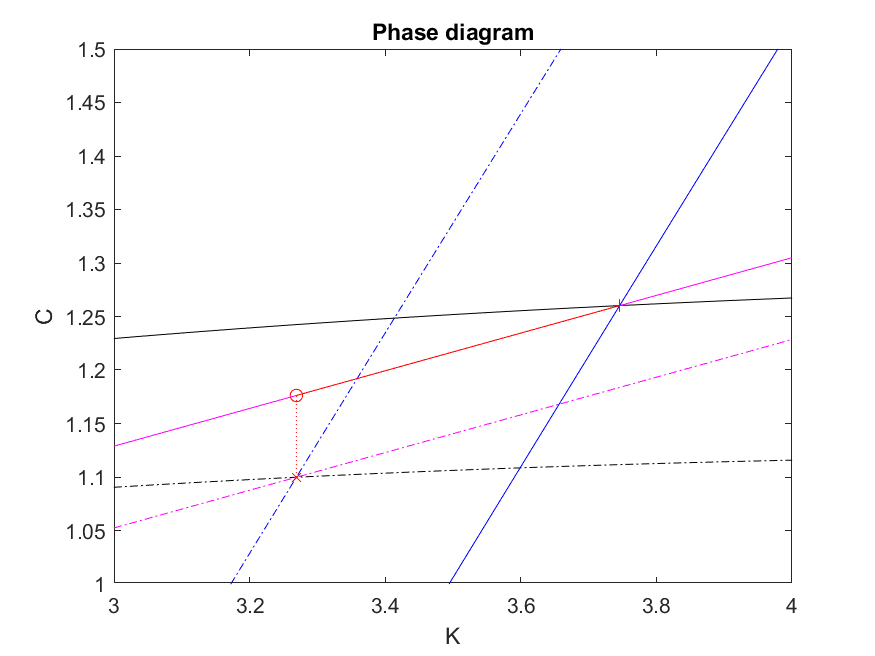
\includegraphics{phase}
The above figure shows the phase diagram as computed via Matlab. The dot-dashed lines show the original, pre-shock, curves for $\Delta k = 0$ (black), $\Delta c = 0$ (blue), and the saddle path (magenta), while the solid lines show the same curves post shock. The system begins at its old steady state (the red x), and then after the shock the system must jump up in $c$ to the new saddle path (jumps to the red o). Then the system will follow the saddle path, tracing out the red line, approaching the new steady state (red $+$) in the limit as $t \rightarrow \infty$.

\subsection{Compute numerically and plot trajectories of $k_t,c_t$ if the productivity shock occurs at $t_0 = 5$ and $z^{'} = z+0.1$.}

We first will compute the new steady state values.\\ From Matlab, $\bar{k}^{'} = 3.7458, \bar{c}^{'} = 1.2602$; $J = \begin{pmatrix} 1.0309 & -1\\ -0.0308 & 1.0299 \end{pmatrix}$. \\
Next, we will diagonalize the system using $J = E\Lambda E^{-1}, \hat{x} = E^{-1}x$:
\begin{align*}
\colvec{2}{\tilde{k_{t+1}}}{\tilde{c_{t+1}}} &= J \colvec{2}{\tilde{k_{t}}}{\tilde{c_{t}}} \\
\Rightarrow \colvec{2}{\hat{k_{t+1}}}{\hat{c_{t+1}}} &= E^{-1} E \Lambda \colvec{2}{\hat{k_{t}}}{\hat{c_{t}}} \\
\Rightarrow \colvec{2}{\hat{k_{t+1}}}{\hat{c_{t+1}}} &= \Lambda \colvec{2}{\hat{k_{t}}}{\hat{c_{t}}}.
\end{align*}
Next, we will write down non-explosive solution for $(\hat{k_t},\hat{c_t})$, and then re-write in terms of the original variables $(k_t,c_t).$

\begin{align*}
\hat{k_{t+1}} &= \lambda_1\hat{k_t} =  1.2060 \hat{k_t}\\
\hat{c_{t+1}} &= \lambda_2\hat{c_t} =  0.8548 \hat{c_t}\\
\Rightarrow \hat{k_{t}} &= c_1 \lambda_{1}^{t}, \hat{c_{t}} = c_2 \lambda_{2}^{t}.
\end{align*}
Our non-explosive solution must have $c_1 = 0$. Re-writing in terms of our original variables,

\begin{align*}
k_t &= e_{1,2} c_2 \lambda_{2}^{t} \\
c_t &= e_{2,2} c_2 \lambda_{2}^{t} \\
\Rightarrow k_{t}^{g} &= e_{1,2} c_2 \lambda_{2}^{t} + \bar{k} \\
\Rightarrow c_{t}^{g} &= e_{2,2} c_2 \lambda_{2}^{t} + \bar{c}.
\end{align*}
Note that we have 2 boundary conditions but only one constant to solve for. We will use our boundary condition for $k$ and solve for an implied initial value of  $c$. We have the following:

\begin{align*}
k_{t_0} &= 3.2690 = 0.9848 c_2 (0.8548)^{5} + 3.7458 \Rightarrow c_2 = -1.0607 \\
c_{t_0} &= 0.1734 (-1.0607) (0.8548)^{5} + 1.2602 = 1.1762.
\end{align*}

We can now write our general solution:
\begin{align*}
k_{t}^{g} &= e_{1,2} c_2 \lambda_{2}^{t} + \bar{k}  = -1.0447 (0.8548)^t + \bar{k}\\
c_{t}^{g} &= e_{2,2} c_2 \lambda_{2}^{t} + \bar{c}  = -0.1840 (0.8548)^t + \bar{c}.
\end{align*}

We will now use our particular solution to compute and plot $k_t,c_t$.

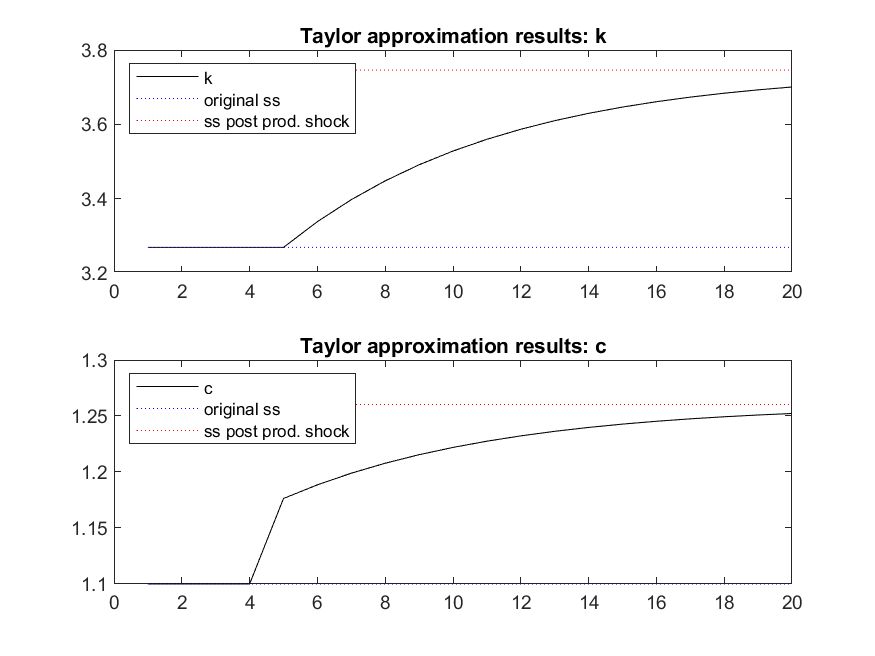
\includegraphics{taylor}

\subsection{Numerically solve the actual transition path using the "shooting method".}

If we put $(k_{t_0},c_{t_0})$ into the nonlinear system  (\ref{eqn:kap}) and (\ref{eqn:con}), we will show that the system does not converge to a steady state:

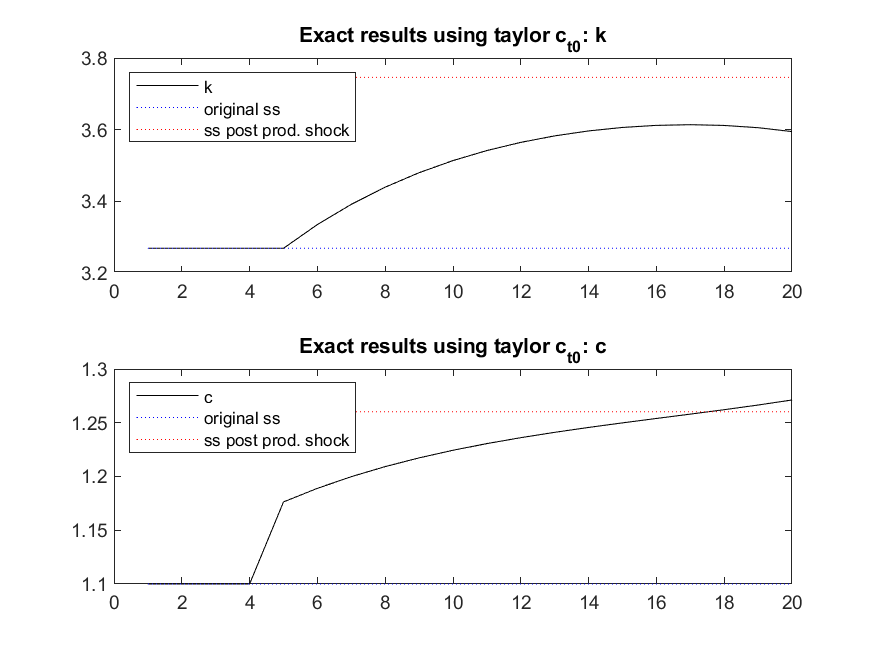
\includegraphics{exact}

Now we will instead use the shooting method to find the actual $c_{t_0}$ needed to converge to the steady state.

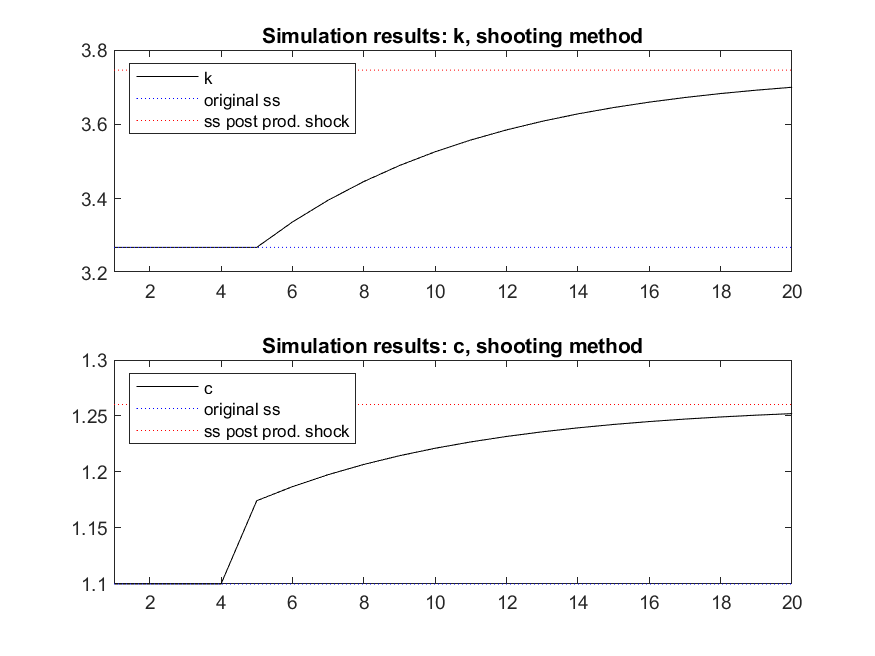
\includegraphics{sh}

\section{Question 2}

We are given three scenarios. For each scenario, we will state the SPP, CP, and CE.

\subsection{Modified 2-period OG model}
In this question we consider a model quite similar to the 2-period OG model we studied in class, but with a few differences as described in the problem set. Since N is constant, WLOG we can set $N=1$. Note that in this question we have two types of consumers. The first are given an allocation in their first period, and the second are given an allocation in the second period. We will number these consumers with the identifiers $1,2$, respectively.

SPP: The social planner maximizes the utilities of the agents given the resource constraint:
\begin{align*} 
&\max_{c_t^{1,t},c_{t}^{1,t-1},c_t^{2,t},c_{t}^{2,t-1}} \text{ ln } c_{t}^{1,t} + \text{ ln } c_{t}^{1,t-1} + \text{ ln } c_{t}^{2,t} + \text{ ln } c_{t}^{2,t-1}\\
&\text{s.t. }  c_{t}^{1,t} +  c_{t}^{1,t-1} + c_{t}^{2,t} +  c_{t}^{2,t-1} \leq \frac{1}{2}w_1 + \frac{1}{2} w_2.
\end{align*}

CP: Each consumer maximizes their own utility over the two periods, subject to their income constraints.
The first type of consumer solves the following maximization problem:
\begin{align*}
&\max_{c_t^{1,t},c_{t+1}^{1,t},M_{t+1}^{1,t}} \text{ ln } c_{t}^{1,t} + \text{ ln } c_{t+1}^{1,t}\\
&\text{s.t. }  p_t c_{t}^{1,t} + M_{t+1}^{1,t} \leq w_1 \\
& \text{and } p_{t+1} c_{t+1}^{1,t} \leq M_{t+1}^{1,t}.
\end{align*}
The next type of consumer solves the following:
\begin{align*}
&\max_{c_t^{2,t},c_{2,t+1}^{t},M_{t+1}^{2,t}} \text{ ln } c_{t}^{2,t} + \text{ ln } c_{t+1}^{2,t}\\
&\text{s.t. }  p_t c_{t}^{2,t}  \leq M_{t+1}^{2,t} \\
& \text{and } p_{t+1} c_{t+1}^{2,t} + M_{t+1}^{2,t}\leq w_2.
\end{align*}

We also have the special case of the initial period. The old in this first period only live for a single period. Those who are given an allocation in this period solve the following maximization problem:
\begin{align*}
&\max_{c_{1}^{2,0},M_1^{2,0}} \text{ ln } c_{1}^{2,0} \\
&\text{s.t. }  p_1 c_{1}^{2,0} + M_{1}^{2,0} \leq w_2.
\end{align*}
Meanwhile, the initial old with no resources solve the following maximization problem:
\begin{align*}
&\max_{c_{1}^{0},M_{1}^{1,0}} \text{ ln } c_{1}^{1,0} \\
&\text{s.t. }  p_1 c_{1}^{1,0} + \leq M_{1}^{1,0} .
\end{align*}

CE: For the competitive equilibtium, prices will adjust so that markets clear, both in the goods market and money market:
\begin{align*}
c_{t}^{1,t} +  c_{t}^{1,t-1} + c_{t}^{2,t} +  c_{t}^{2,t-1} &= \frac{1}{2}w_1 + \frac{1}{2} w_2 \\
M_{t+1}^{1,t} + M_{t+1}^{2,t} &= M.
\end{align*}

\subsection{3-period OG model}
We consider an OG model consisting of agents that live 3-periods. This time, generation sizes are no longer necessarily fixed.

SPP: The social planner maximizes the utilities of the agents given the resource constraint: 
\begin{align*}
&\max_{c_t^{t},c_{t}^{t-1},c_{t}^{t-1}} N_{t}\text{ ln } c_{t}^{t} + N_{t-1}\text{ ln } c_{t}^{t-1} + N_{t-2}\text{ ln } c_{t}^{t-2}\\
&\text{s.t. }  N_{t}c_{t}^{t} +  N_{t-1}c_{t}^{t-1} + N_{t-2}c_{t}^{t-2}\leq N_{t}w_1 + N_{t-1}w_2 + N_{t-2}w_3.
\end{align*}


CP: Outside of the initialization, agents solve the following maximization problem:
\begin{align*}
&\max_{c_t^{t},c_{t+1}^{t},c_{t+2}^{t},M_{t+1}^{t},M_{t+2}^{t}} \text{ ln } c_{t}^{t} + \text{ ln } c_{t+1}^{t}+ \text{ ln } c_{t+2}^{t}\\
&\text{s.t. }  p_t c_{t}^{t} + M_{t+1}^t \leq w_1 \\
& \text{and } p_{t+1} c_{t+1}^t  + M_{t+2}^t \leq  w_2 + M_{t+1}^t \\
& \text{and } p_{t+2} c_{t+2}^t \leq w_3 + M_{t+2}^t.
\end{align*}

We next must consider the initial case. There are 2 'special' generations (i.e. generations which live less than 3 periods). First we will consider the 2-period generation. They solve the following maximization problem:
\begin{align*}
&\max_{c_{1}^{0},c_{2}^{0},M_{2}^{0}}  \text{ ln } c_{1}^{0}+ \text{ ln } c_{2}^{0}\\
& \text{s.t. } p_{1} c_{1}^0  + M_{2}^0 \leq  w_2 \\
& \text{and } p_{2} c_{2}^0 \leq w_3 + M_{2}^0.
\end{align*}
Finally, we also consider the 1-period generation. They solve the following:
\begin{align*}
&\max_{c_{1}^{-1},M_{1}^{-1}}  \text{ ln } c_{1}^{-1}\\
& \text{s.t. } p_{1} c_{1}^{-1} \leq w_3.
\end{align*}

CE: For the competitive equilibtium, prices will adjust so that markets clear, both in the goods market and money market:
\begin{align*}
N_{t}c_{t}^{t} +  N_{t-1}c_{t}^{t-1} + N_{t-2}c_{t}^{t-2} &= N_{t}w_1 + N_{t-1}w_2 + N_{t-2}w_3.\\
M_{t+1}^{t} + M_{t+1}^{t-1} &= M.
\end{align*}

\subsection{Cake eating problem}
We now consider a single agent, given an allocation in period 1, with perfect storage. In this case, the SPP, CP, and CE all collapse to a single optimization problem.

The single agent solves the following maximization problem:

\begin{align*}
&\max_{ c_{i}, i \in \mathbb{N}}  \sum_{t=1}^{\infty}\beta^{t} u(c_t)\\
& \text{s.t. } \sum_{t=1}^{\infty} c_t = k_1\\
& \text{and } c_i \geq 0 \forall i \in \mathbb{N}.
\end{align*}

\end{document}
